\documentclass{article}
% \usepackage{showframe}
\usepackage{siunitx}
\usepackage{booktabs}
\usepackage{graphicx}
\usepackage{amsmath}
\usepackage{mathtools}
% \usepackage{minted}
\usepackage{tabularx}
\usepackage{url}
% \usepackage{subfig}
% \usemintedstyle{xcode}

% \usepackage{fullpage}

\frenchspacing
% \setlength{\parindent}{0ex}
% \setlength{\parskip}{3 ex plus 2 ex minus 1 ex}

\title{Homework 9}
\author{Josh Bradt}
\date{April 18, 2016}

\begin{document}

\maketitle

\section{Models}

    Multiplying an $n \times m$ matrix by a vector of length $m$ should take
    \begin{align}
        \mathcal{M} &= mr + nm (2r+2c) + mw \nonumber \\
                    &= \frac{2m^2}{p} (r+c) + 2mr
    \end{align}
    where $r$ is the memory access time, $p$ is the number of processes, and $c$ is the time per floating point operation. To simplify the first line, I took advantage of the fact that $n = m / p$, and I assumed that memory reads and writes took the same amount of time. The Blue Waters documentation\footnote{\url{https://bluewaters.ncsa.illinois.edu/node_core_comparison}} lists a per-core performance of \SI{19.6}{GFLOPS} and a peak memory access speed of \SI{102}{GB/s}. This suggests that the values of the two parameters here are $c = 1 / (\SI{19.6}{GFLOPS}) = \SI{5.1e-11}{s}$ and $r = (\SI{8}{B}) / (\SI{102}{GB/s}) = \SI{7.8e-11}{s}$. (Note that this is probably an unrealistically optimistic estimate\dots).

    The communication time per vector chunk is given by
    \begin{equation}
        \mathcal{C} = R n = \frac{Rm}{p}.
    \end{equation}
    Here, $R$ is the communication rate, which I found to be \SI{6.8e-10}{s/B} on the last assignment.

    This means that the total time for the method using \texttt{MPI\_Allgather} should be
    \begin{equation}
        T_\text{AG} = p \mathcal{C} + \mathcal{M}
    \end{equation}
    since each process must send one chunk and receive the remaining $p-1$ chunks before performing the multiplication.

    The total time for the ring method should be
    \begin{equation}
        T_\text{ring} = p \max\left(\mathcal{C}, \frac{\mathcal{M}}{p}\right).
    \end{equation}
    That is, the total time taken is the time taken by the slower of the two overlapping procedures.

\section{Results}

    I wrote my own code to perform a matrix-vector multiplication using MPI with the two implementations described in the assignment. I compiled the code on Blue Waters with the default compiler and MPI implementation, and I ran all of the tests in one job. The job requested 64 XE nodes. I ran using the command \texttt{aprun -n \$NPROC -N 16 -e MPICH\_NEMESIS\_ASYNC\_PROGRESS=1 -e MPICH\_MAX\_THREAD\_SAFETY=multiple ...} where \texttt{\$NPROC} represents the total number of processes to use in a given run. The data is listed in Table~\ref{tab:results} and plotted along with the models in Figure~\ref{fig:results}.

    The results were not entirely what I expected. Both the measurements and the models show little difference between the two methods, while I had assumed that the ring communication method would be significantly faster since it overlaps communication and computation. The models, however, show that the computation time grows with matrix size $m$ as $O(m^2)$ while the communication time only grows as $O(m)$, which supports the idea that the communication time is insignificant compared to the computation time for large $m$.

    Based on these results, I would probably choose the method based on \\\texttt{MPI\_Allgather} in most cases since it is much simpler and less error-prone.


    \begin{table}
    \centering
    \begin{tabular}{S[table-format=6]
                    S[table-format=4]
                    S[table-format=3]
                    S[table-format=1.4e+2]
                    S[table-format=1.4e+2]}
    \toprule
    {Matrix Size} & {Num. proc.} & {Chunk size} & {Allgather time [s]} &  {Ring time [s]}  \\
    \midrule
    1024          &  128         & 8            & 6.5088e-05           &  4.1914e-04       \\
    16384         &  128         & 128          & 1.0182e-02           &  1.0066e-02       \\
    102400        &  128         & 800          & 4.3615e-01           &  3.6520e-01       \\
    1024          &  256         & 4            & 4.0102e-04           &  8.3899e-04       \\
    16384         &  256         & 64           & 5.8219e-03           &  5.7230e-03       \\
    102400        &  256         & 400          & 2.2142e-01           &  1.7744e-01       \\
    1024          &  512         & 2            & 9.5201e-04           &  1.8370e-03       \\
    16384         &  512         & 32           & 3.6731e-03           &  3.7570e-03       \\
    102400        &  512         & 200          & 1.1294e-01           &  8.9725e-02       \\
    1024          &  1024        & 1            & 1.4019e-04           &  3.8991e-03       \\
    16384         &  1024        & 16           & 2.2910e-03           &  4.2529e-03       \\
    102400        &  1024        & 100          & 5.7398e-02           &  4.7342e-02       \\
    \bottomrule
    \end{tabular}
    \caption{Results}
    \label{tab:results}
    \end{table}

    \begin{figure}
        \centering
        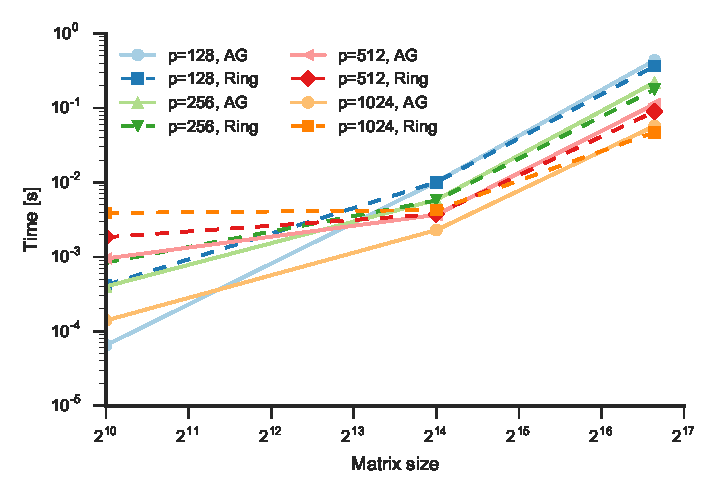
\includegraphics{data.pdf}\\
        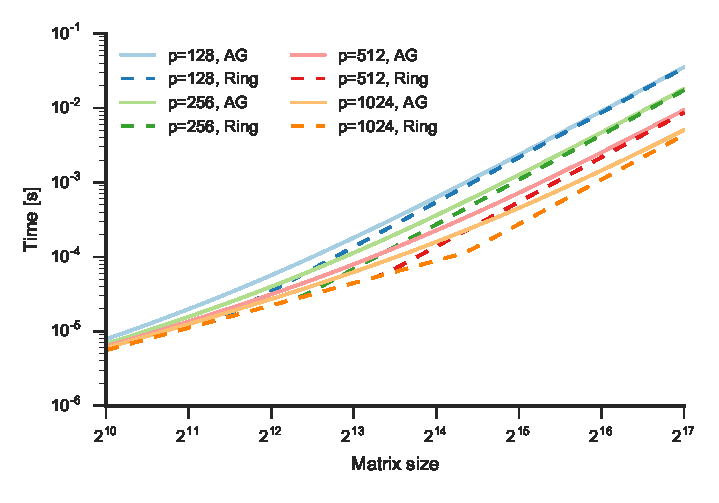
\includegraphics{model.pdf}
        \caption{The measured results from the experiment (top) and the models of the expected performance (bottom).}
        \label{fig:results}
    \end{figure}

\end{document}
